\section{Model assessment}\label{subsec:Cost}
\subsection{The Rate of True-Positve - ROC Curve}\label{subsec:AUC}
A \ac{ROC} curve is a tool used to measure and visualize a binary classifiers' ability 
to predict trends. In figure \ref{fig:ROC} I have plotted an illustration of a \ac{ROC} curve.
The curve is plotted on an x-, y-axis where the x-axis represents 
false-positive rates and the y-axis represents true-positive. The different values 
for the curve are the rate of true positives with different thresholds, i.e. 
the value deciding whether an event is 1 or 0, signal or background. If a classifier 
has learned nothing and is simply guessing, the \ac{ROC} curve will be a linear curve 
going from 0 to 1. This line is often drawn in \ac{ROC} curve. The better the 
classifier is, the higher the \ac{ROC} curve will bend towards the upper-left corner of the 
graph. The worse it is, the more it will bend to the lower right corner. 
\\
A metric often used to measure a classifiers' ability create an output which effectively 
separates two categories, is the \ac{AUC}. The higher the area, the larger the separation. 
An ideal classifier which perfectly separates two categories will achieve a \ac{AUC} of 1.
A classifier which simply guesses, will achieve an \ac{AUC} of 0.5. Both this cases assume 
an equal weighting of both signal and background. 
\begin{figure}
    \centering
    \makebox[0.75\linewidth][c]{%
    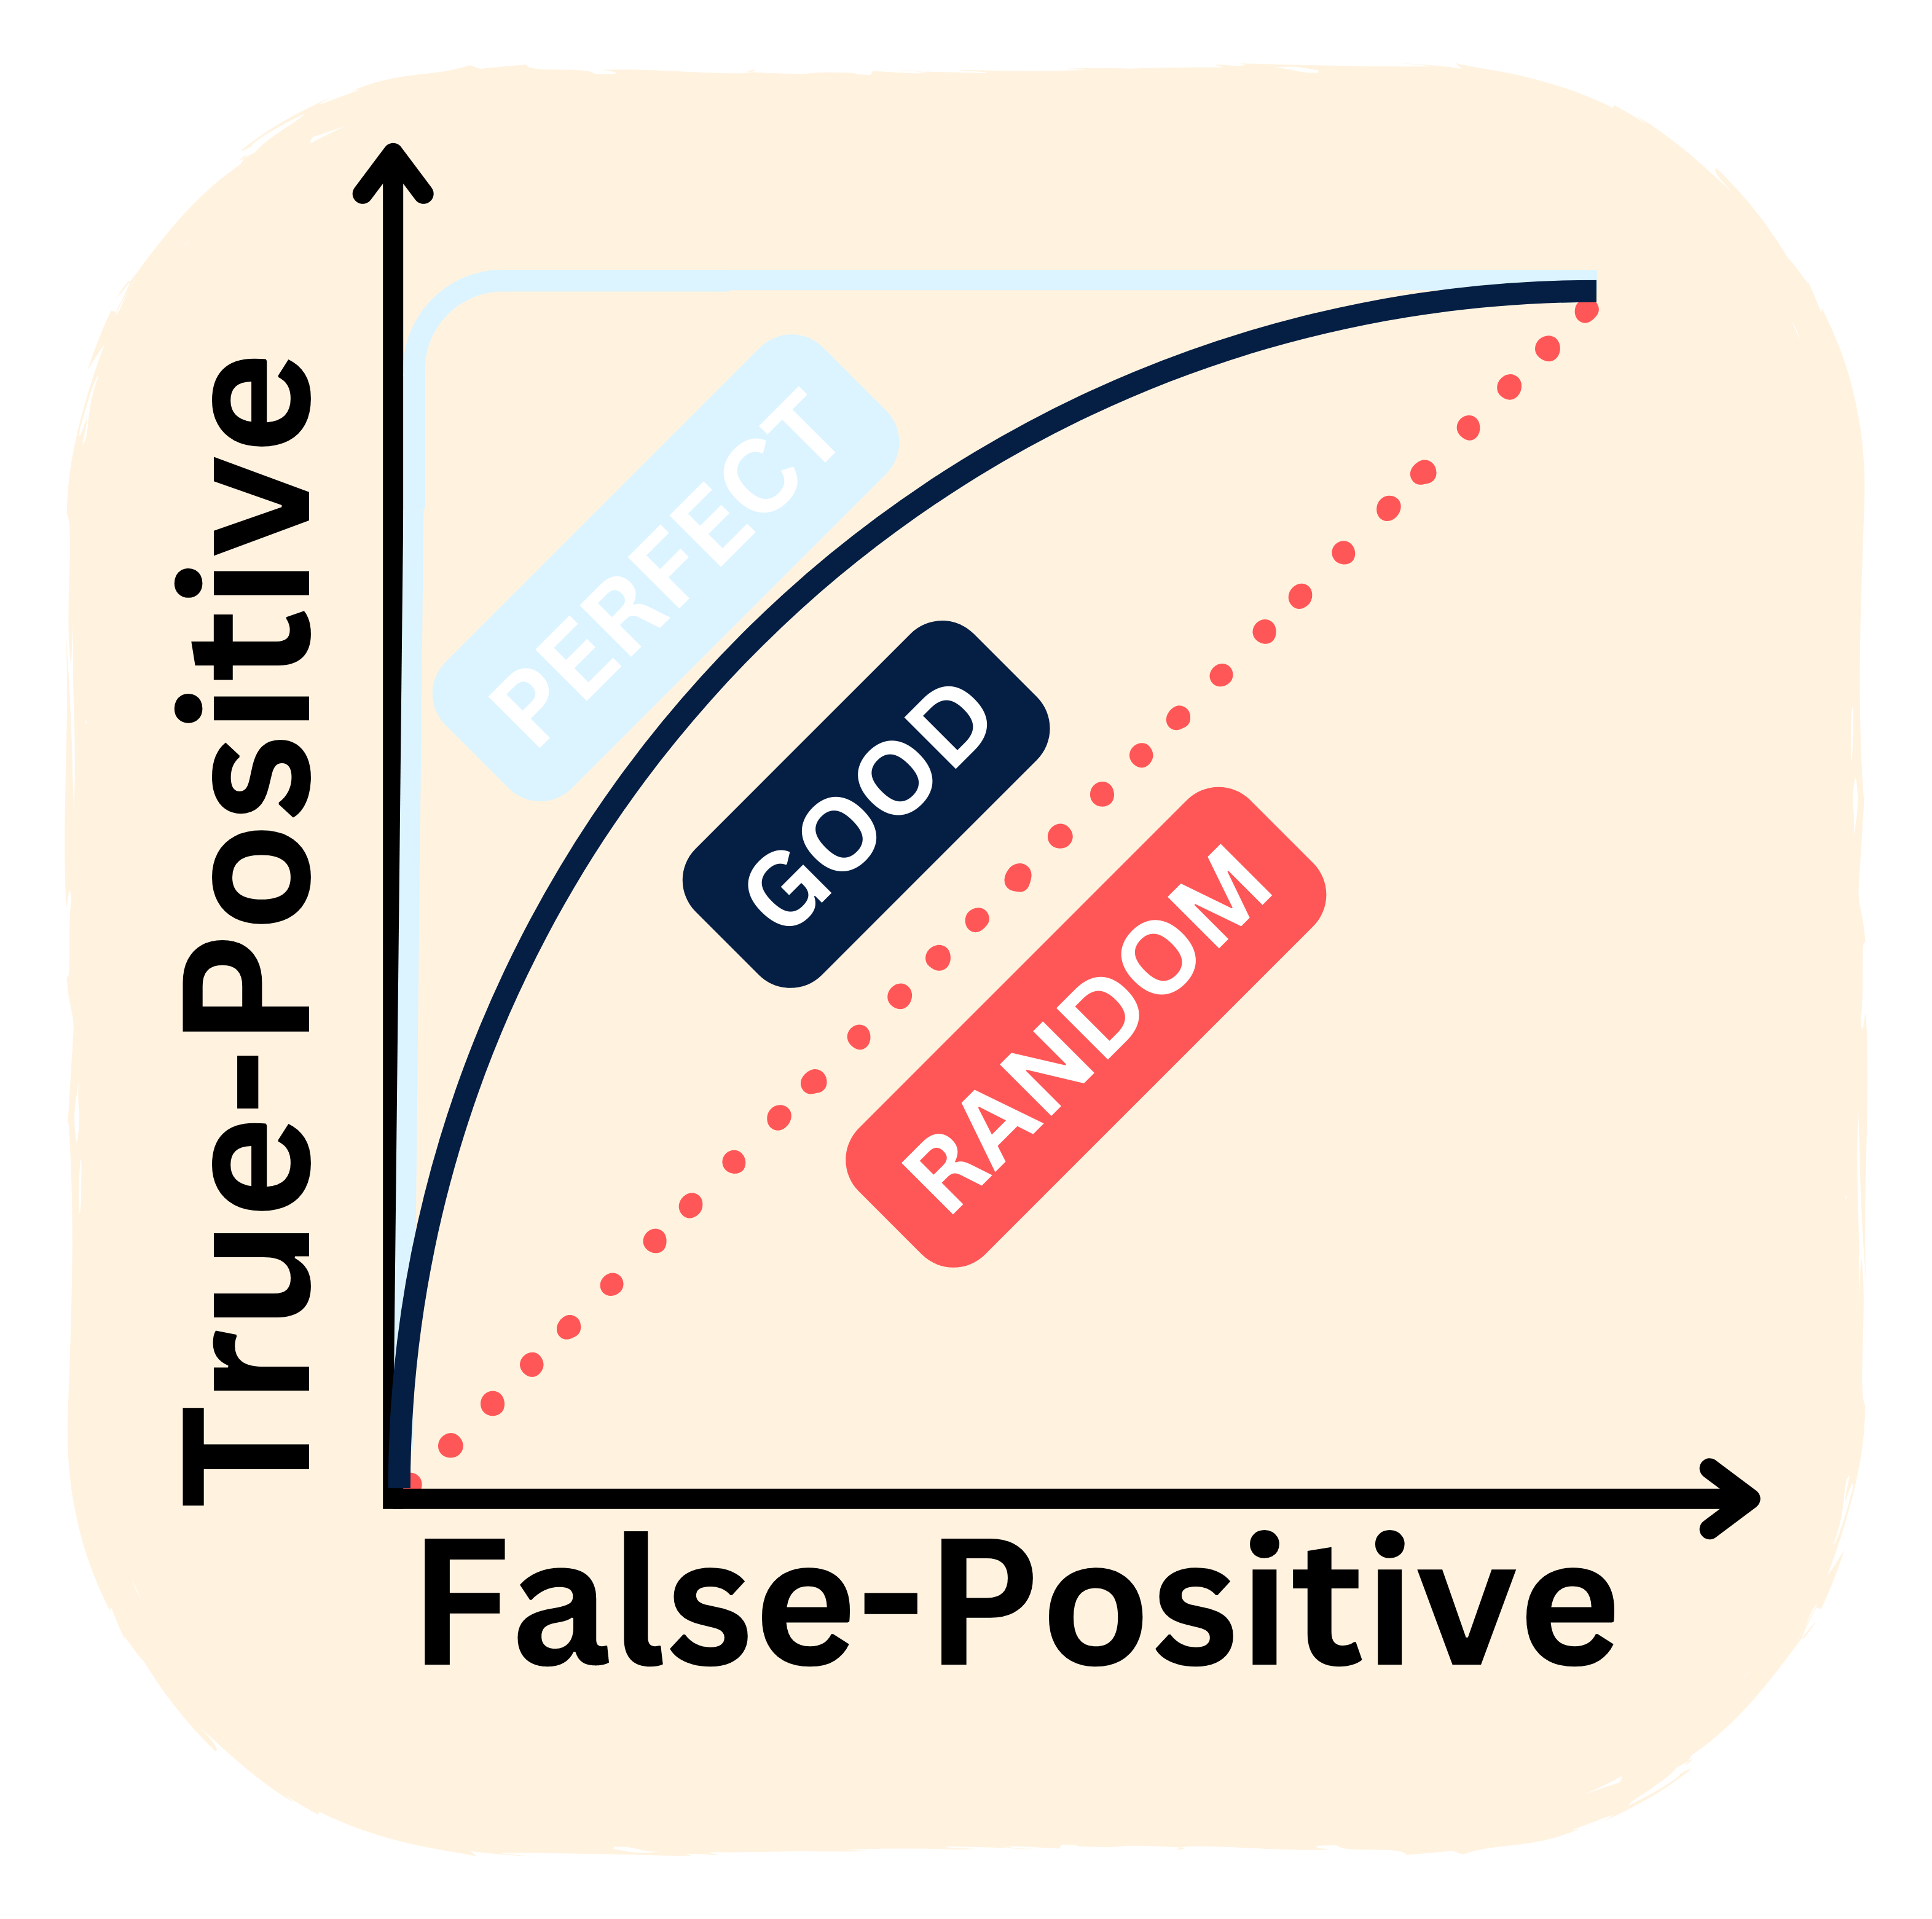
\includegraphics[width=0.45\textwidth]{Figures/Illustrations/True-Positive.png}
    }
    \caption{An illustration of a ROC curve.}
    \label{fig:ROC}
\end{figure}
\subsection{Sensitivity}\label{subsec:Sensitivity}
\ac{AUC} is a very good measure of how separated the distribution for signal and background are 
for a feature. In the search for new physics, features with large separation between signal and background
are incredibly helpful, but not the end goal. The final result in the search for new physics is the discovery 
of a significant deviation between the \ac{SM} and experiment. We measure the deviation between the measured 
collision data and the simulated \ac{SM} data in units of significance, Z. 
\\
For a given signal region with $n_{obs}$ events of measured collision data and b simulated \ac{SM} data, we define
the significance of a deviation as
\begin{align}
Z=\sqrt{2\left[n_{\text {obs }} \ln \frac{n_{\text {obs }}}{b}-n_{\mathrm{obs}}+b\right]} \text { or } 
Z=\sqrt{2\left[(s+b) \ln \left(1+\frac{s}{b}\right)-s\right]}, 
\end{align}
where we have defined the signal, s as $s = n_{obs} - b$. In the case of large statistics ($b>>s$), we can write Z 
as 
\begin{align}\label{eq:Z}
    Z=\frac{n_{o b s}-b}{\sqrt{b}} = \frac{s}{\sqrt{b}}.
\end{align}
By studying equation \ref{eq:Z} we observe that the significance resembels the ration for signal and background. The 
larger the Z, the more significant the deviation. In physics, one often deems the results a discovery if Z is larger than 5.  
\\
In the case we are not intrested in discovering physics, but simple to measure the sensitivity of a model, we can also use 
significance. In this case we do not have $n_{obs}$. Instead we simply define s as the number of events for the simulated signal 
inside the signal region. This number would be spesific for each mass combination and will be a measure for how sensitive 
the model is for that exact combination. 